\documentclass[journal]{IEEEtran}
\usepackage[utf8]{inputenc}
\usepackage[T1]{fontenc}
\usepackage{amsmath,amssymb,booktabs,array,tabularx,multirow,graphicx,xcolor,hyperref,algorithm,algpseudocode,tikz,cite}
\usetikzlibrary{positioning,arrows.meta,fit,calc}
\graphicspath{{../results_final/plots/}}
\hypersetup{hidelinks}
\newcommand{\ck}{\checkmark}
\markboth{SINGH: RELIABILITY-AWARE DFT FOR AUTONOMOUS ROBOTIC SOCS}{}
\begin{document}
\title{Reliability-Aware Design-for-Test Scheduling for Autonomous Robotic SoCs: Literature Review and Behavioral Prototype}
\author{Ashmit Singh%
\thanks{A. Singh is with the Department of Electronics and Electrical Engineering (VLSI Design and Technology), Vellore Institute of Technology, Vellore, India.}}
\maketitle

\begin{abstract}
Conventional design-for-test (DFT) for systems-on-chip (SoCs) -- scan insertion, automatic test pattern generation (ATPG), and memory built-in self-test (MBIST) -- is organized around a single manufacturing-time objective: maximize defect coverage per unit test time and per unit test-access-mechanism (TAM) bandwidth. Autonomous robotic SoCs, in contrast, must remain trustworthy across an operational lifetime during which aging (NBTI/HCI-induced delay degradation), transient/soft errors, and mission-driven duty cycles change the reliability picture continuously. This paper reviews the literature across four layers that bear directly on this problem: (i) conventional SoC test-architecture and scheduling theory, (ii) aging-aware reliability monitoring, (iii) in-field/online and concurrent testing, and (iv) criticality- and state-aware scheduling of non-test workloads on heterogeneous SoCs, with the closest academic analogue being mission-aware task scheduling for autonomous-vehicle SoCs. We synthesize what each family of techniques assumes, whether its decisions are static or adaptive, and whether it is manufacturing-only or field-capable. We then construct a literature-gap matrix and argue -- cautiously, and only to the extent the surveyed literature supports it -- that while aging monitoring, in-field self-test, and criticality-aware scheduling each exist independently and some pairwise combinations exist in industrial prior art, the joint fusion of live aging/health state, operating-mode state, and per-block criticality into a single runtime DFT scheduling decision for a robotic (non-automotive, non-always-active) SoC is not demonstrated in the sources examined here. This motivates, but does not by itself validate, a reliability-aware adaptive DFT scheduler as a research direction. A behavioral prototype of the proposed scheduler and its preliminary single-seed results are reported in Section~\ref{sec:impl}; they do not establish silicon-level claims.
\end{abstract}

\begin{IEEEkeywords}
Design-for-testability, system-on-chip testing, aging-aware testing, NBTI, HCI, in-field self-test, online testing, test scheduling, functional safety, ISO 26262, autonomous robotic SoC.
\end{IEEEkeywords}

\section{Introduction and Theoretical Foundations}
\subsection{Motivation}
Modern SoCs integrate heterogeneous compute, memory, and I/O cores whose combined defect surface and post-silicon reliability risk have grown faster than the test infrastructure historically used to manage them. Design-for-testability (DFT) -- principally scan chains, ATPG-generated stuck-at and transition-delay pattern sets, and MBIST for embedded memories -- was developed to solve a manufacturing-time problem: given a fixed test budget (automatic test equipment (ATE) time, TAM width, tester memory depth), maximize fault coverage before the part ships \cite{r1,r2}. This is fundamentally an offline, one-shot optimization: the test schedule is computed once, against a test-access architecture that is itself co-optimized for the same fixed objective \cite{r3}.

Autonomous robotic systems change the operating assumption. A robotic controller SoC executes continuously, in physically uncontrolled environments, over a service life measured in months or years rather than in ATE seconds. Over that life, negative-bias temperature instability (NBTI) and hot-carrier injection (HCI) progressively shift transistor threshold voltages and increase gate delay \cite{r4,r5,r6,r7}; transient/soft errors accumulate stochastically during operation \cite{r8}; and the SoC's own workload -- idle, actively executing a motion-control loop, or degraded after a fault flag -- changes what fraction of its resources can be spared for testing at any given moment. A test schedule computed once, at manufacturing time, against none of this information cannot, by construction, respond to it.

\subsection{Why Static DFT Is Insufficient by Itself}
Two independent bodies of work already relax the ``test once, at manufacturing time'' assumption, but each relaxes it along only one axis:
\begin{itemize}
\item \textbf{Aging-aware monitoring} instruments a chip with delay/aging sensors, typically placed using a static-timing-analysis (STA) ranking of paths most likely to become critical under NBTI/HCI, and reports a live degradation signal \cite{r4,r5,r6}. This gives health information but does not by itself decide when or how to re-test.
\item \textbf{In-field self-test controllers}, exemplified by patented automotive practice, schedule LBIST/MBIST at power-up, at shutdown, and periodically during runtime to satisfy functional-safety standards such as ISO 26262 \cite{r9,r10}. This gives a runtime test trigger but, in the disclosed mechanism, the trigger is largely periodic/event-based rather than continuously informed by a fused reliability-plus-workload-state signal.
\end{itemize}
Neither line of work, on its own, produces a scheduler whose test depth, frequency, and target block are jointly driven by (a) live aging/health state, (b) the SoC's current operating mode, and (c) the safety criticality of the block in question. Section~\ref{sec:gap} returns to this point with a literature-gap matrix; the introduction here is deliberately phrased as a motivating observation, not a novelty claim.

\subsection{Theoretical Foundations}
This subsection fixes notation and terminology used throughout the survey.

\textbf{Scan and ATPG.} A scan chain reconfigures sequential elements into a shift register during test mode, giving external controllability/observability of internal state. ATPG generates input vectors targeting a fault model -- commonly single stuck-at and transition-delay faults -- and reports fault coverage $FC$, the fraction of modeled faults detected by the pattern set.

\textbf{Test-access architecture.} For a modular SoC, wrappers (e.g., IEEE 1500-style) isolate each core and test-access mechanisms (TAMs) route pattern data between the ATE (or on-chip pattern source) and the wrapped cores. Goel and Marinissen formulate joint wrapper/TAM design as an optimization that partitions a fixed total TAM width $W$ among $N$ cores to minimize the SoC test time $T_{test}$, and derive an architecture-independent lower bound on $T_{test}$ for a given $W$ \cite{r1}.

\textbf{Test scheduling.} Given a set of test tasks (one or more per core) with fixed durations and a set of shared test resources, test scheduling assigns start times to tasks so that the makespan is minimized subject to resource and (optionally) power/thermal constraints. Chakrabarty shows this problem is equivalent to $m$-processor open-shop scheduling, hence NP-complete for $m>2$, and gives an exact mixed-integer linear programming (MILP) formulation together with a shortest-task-first heuristic for larger instances \cite{r2}. He et al. extend scheduling to a thermal constraint, partitioning long test sets into shorter sequences separated by cooling intervals so that no core under test exceeds a temperature limit while test time is still minimized \cite{r3}. Both are still static: the schedule is one fixed sequence of start times computed offline from known test-set durations and a known resource/thermal model, not information available only at runtime.

\textbf{Aging mechanisms.} NBTI affects PMOS transistors under negative gate bias, gradually increasing $|V_{th}|$ and hence gate delay; HCI has an analogous effect driven by channel hot-carrier trapping, more prominent in NMOS devices and under high switching activity. Both mechanisms are cumulative and workload/stress dependent, so the paths that become timing-critical after some months of operation are not necessarily the paths that were critical at time zero \cite{r4,r5}. This motivates placing dedicated aging/delay sensors specifically on paths predicted -- via STA under a stress model -- to become critical, rather than instrumenting the whole design, since full instrumentation is area- and power-prohibitive \cite{r4}.

\textbf{Fault models relevant to reliability.} Beyond the manufacturing-time stuck-at and transition-delay models, a reliability-oriented evaluation must additionally consider: (i) delay-degradation faults, where a path that passed at time zero fails timing after aging; (ii) transient/soft errors from particle strikes or noise, which are not permanent and require repeated or continuous monitoring rather than a one-shot test \cite{r8}; and (iii) intermittent faults, whose detection probability depends on operating condition (voltage, temperature) at the moment of test.

\textbf{Dynamic power.} Where a power formulation is required for test-power or test-scheduling discussion, the standard first-order dynamic-power model is
\begin{equation}
P_{dynamic}=\alpha C V_{dd}^{2} f,
\end{equation}
where $\alpha$ is the switching activity factor, $C$ the switched capacitance, $V_{dd}$ the supply voltage, and $f$ the clock frequency. Test-mode switching activity is typically much higher than functional-mode activity because scan shift toggles many non-functional states, which is the reason low-power DFT techniques such as scan-chain reordering and X-filling exist \cite{r11}: they choose don't-care (X) bit assignments and cell orderings that reduce $\alpha$ during shift without altering the fault set covered.

\textbf{Reliability and criticality metrics.} At the system level, functional-safety practice (ISO 26262) defines quantitative metrics -- the Single-Point Fault Metric (SPFM), Latent Fault Metric (LFM), and Probabilistic Metric for random Hardware Failures (PMHF) -- that constrain how much of a design's fault space may go undetected, as a function of the Automotive Safety Integrity Level (ASIL) assigned to a function \cite{r10}. These metrics are defined at the standard level and are used in this survey only as evaluation-framing vocabulary; no specific published SPFM/LFM/PMHF numerical result is attributed to any of the DFT papers surveyed here, since none of the verified sources reports them.

\section{Conventional DFT and SoC Test Architectures}
Goel and Marinissen address the SoC test-architecture design problem directly: given a set of cores, each with one or more scan-based tests of known length, and a fixed total TAM width, determine (i) how many TAMs to instantiate, (ii) each TAM's width, (iii) the assignment of cores to TAMs, and (iv) for cores with flexible-length scan chains, how to balance the chains -- so as to minimize the SoC-level test time \cite{r1}. The paper's central contribution is an architecture-independent heuristic that is reported to come close to a derived theoretical lower bound on test time across the ITC'02 SoC benchmark suite. This is a purely manufacturing-time, defect-oriented optimization: it has no notion of in-field operation, aging, or workload state, and none is claimed.

Chakrabarty's MILP formulation for test scheduling assumes a fixed test-resource graph (e.g., dedicated or shared BIST engines, test buses) and fixed, precomputed test-set durations per core, and computes an optimal start-time assignment offline \cite{r2}. Because exact MILP solving does not scale, a shortest-task-first heuristic is also given for larger core counts. The scheduling decision is entirely static: once computed, it is not revisited in response to any signal generated after manufacturing.

He et al. add a physical constraint -- junction temperature -- to the same class of problem, partitioning each core's test set into shorter sequences with inserted cooling gaps, and interleaving sequences from different cores so that TAM bandwidth is not wasted during a cooling gap \cite{r3}. The scheduling problem is again solved offline (the authors use constraint logic programming), against a thermal model that is fixed before the schedule is generated; the resulting schedule does not adapt to a chip's actual, individual thermal or aging trajectory in the field. Rosinger et al. independently formulate a closely related thermal-safe scheduling problem and report a heuristic that approaches an ILP-derived lower bound on test time under the same class of temperature constraint \cite{r12}; it is added here purely as corroboration that the thermal-constrained scheduling result is not an isolated finding, not as a distinct axis of the taxonomy.

\textbf{Assumptions common to this family.} All three works in this section assume: (a) the test is performed once, at manufacturing/production test time, by an external ATE or an on-chip controller invoked in a manufacturing-like flow; (b) the objective is test time and/or TAM/area cost, not in-field reliability; and (c) the fault model is exclusively the manufacturing-time model (stuck-at, transition-delay). None incorporates aging, live system state, or block criticality, because none was designed to.

\section{Low-Power and Power-Constrained DFT}
Scan-based testing typically induces switching activity far above functional-mode levels, which raises test power, can create IR-drop-induced yield loss, and -- relevant here -- couples to the thermal constraint discussed in Section~II, since higher shift power raises junction temperature during test. Seo et al. address scan shift power directly with a scan-chain-reordering-aware X-filling and stitching method: don't-care bits in the ATPG-generated test cubes are filled, and scan cells are ordered and stitched, jointly, so that adjacent scan-cell values during shift are more likely to match, reducing shift-toggle activity without adding dedicated low-power hardware and without changing the covered fault set \cite{r11}.

\textbf{Relevance to the target architecture.} This family is orthogonal to, and compatible with, the aging-aware and adaptive-scheduling layers discussed next: a reliability-aware scheduler that decides when and how deep to test a block still benefits from having that block's underlying scan/BIST primitives be power-efficient, since a runtime test that spikes power or temperature is precisely the kind of disruption an operating robotic system with a live mission cannot always absorb. No claim of adaptivity, aging-awareness, or criticality-awareness is made for, or by, this family of techniques; its role is a power/thermal-efficiency substrate under whatever schedule decides to invoke it.

\section{Reliability-Aware DFT and Aging Monitoring}
Three verified sources define this layer directly.

G\'omez and Champac propose a pre-layout, statistical methodology for choosing where to insert aging/delay sensors: rather than requiring post-layout spatial-correlation information (unavailable early in the design flow), the method estimates, from a stress-probability model of NBTI (and, where relevant, process-variation) degradation, which paths are statistically likely to become critical, and places sensors to maximize coverage of that predicted critical-path set \cite{r4}. A subsequent journal extension by the same authors formalizes this as an ``early selection of critical paths'' procedure and reports the predicted sensor placement's coverage against a spatial-correlation-informed placement, using a first-order NBTI threshold-voltage-shift model of the form $\Delta V_{th,NBTI}=(1-S_v\Delta V_{th,PV})A\alpha^{n}t^{n}$, where $A$ and $S_v$ are fitted technology constants, $\alpha$ is duty-cycle-dependent stress probability, and $t$ is stress time \cite{r5}.

A closely related pre-layout methodology is given by V\'azquez et al., who extend the sensor-placement problem to jointly account for process-variation (PV) and aging (NBTI) effects, arguing that PV-only or aging-only placement heuristics under-cover the true set of paths that become critical once both effects are combined \cite{r13}. This is the paper referred to as an aging-sensor placement reference in the project's frozen specification; it is complementary to, and independently verifiable from, the G\'omez--Champac line of work above, and is treated here as a distinct source rather than merged into it. Firouzi et al. address a related but distinct problem -- selecting a representative subset of critical paths for delay-monitor placement under combined aging and variation, so that a limited sensor budget still tracks the dominant degradation modes -- and report their aging- and variation-aware selection heuristic on standard benchmark circuits \cite{r14}; this paper is verified separately from G\'omez et al. and V\'azquez et al. despite the topical overlap, since it targets sensor selection under a budget rather than early-design-phase path prediction.

Koneru et al. take a complementary, runtime approach: rather than predicting aging offline, they monitor run-time stress directly using existing DFT infrastructure (scan-based delay measurement) to produce a fine-grained, per-chip aging prediction that tracks the actual stress history of the individual die rather than a population-average model \cite{r6}. A subsequent journal extension replaces the original prediction step with a support-vector-regression model trained offline on captured stress samples, improving prediction accuracy without changing the underlying DFT-infrastructure-reuse principle \cite{r15}. This is architecturally significant for the present survey because it demonstrates that DFT hardware can be reused as a sensing channel for reliability information, not only as a manufacturing-test channel -- exactly the reuse a reliability-aware runtime scheduler would depend on.

Yu et al. address a closely related but distinct problem: production-test-time aging screening. Their ZeroScreen architecture performs a fast, pattern-based, time-zero aging prediction so that devices can be binned by predicted reliability margin before shipment, with a reported per-device screening time on the order of 8~ms at a 50~MHz test clock \cite{r7}. This is a manufacturing-time technique -- it screens devices once, before deployment -- and is included here because it establishes that aging-aware prediction models are mature enough to be integrated into a production test flow, which is a necessary (but not sufficient) precondition for using an analogous model as a live input to an in-field scheduler.

\textbf{Common structure and gap.} All of the sensor-placement and runtime-monitoring works verified in this section \cite{r4,r5,r13,r14,r6,r15,r7} produce a health/aging signal -- whether pre-layout-predicted, runtime-monitored, or production-screened -- but none couples that signal to a scheduling decision about which block to test next, how deeply, or how often, in response to the system's current operating mode. They are inputs a scheduler could consume; none of them is a scheduler.

\section{In-Field and Online Testing}
Two verified sources anchor this layer, one industrial/patented and one academic/asynchronous-logic-specific.

Jain et al.'s patented in-field self-test controller (assigned to Qualcomm) is explicitly motivated by ISO 26262's requirement that safety-related automotive electronic systems be checked for structural hardware faults throughout their operational life, not only at manufacturing \cite{r9,r10}. The disclosed controller stores encoded test patterns in on-chip ROM, decodes them through a memory-data finite-state machine, and drives logic-BIST (LBIST) and memory-BIST (MBIST) cores via a JTAG interface at three defined points: system power-up, periodically during runtime, and at shutdown initiation. This is, to the best of the authors' knowledge based on the sources examined, the closest industrial prior art to an ``in-field, periodically triggered DFT controller,'' and it establishes that in-field self-test scheduling triggered by system lifecycle events -- as opposed to only by ATE commands -- is already patented, non-novel territory. Two limitations are notable for the present research direction: (i) the disclosed triggers are lifecycle/periodic, not continuously reliability-state-dependent, and (ii) the target domain is automotive, where the vehicle is reasonably modeled as ``on'' for the duration of a drive cycle, which does not match a robotic controller's more heterogeneous idle/active/degraded duty cycle.

Maier and Steininger address online testing at the circuit level for asynchronous logic, proposing a Concurrent Built-In Self-Test (CBIST) technique that exploits the unproductive ``NULL phase'' of a standard four-phase asynchronous handshake protocol to interleave test-vector processing with normal data processing, achieving a fully transparent, fully concurrent test with no interruption to functional operation \cite{r16}. This is valuable to the taxonomy as a concrete existence proof that concurrent (as opposed to periodically interrupting) online test is achievable in principle, though the technique as published targets asynchronous-logic test infrastructure specifically and does not address reliability-state-driven scheduling of which block or how deep to test. the primary peer-reviewed publication is the 17th IEEE DDECS symposium (2014), and the arXiv record is a later self-archived copy of the same result -- both are now correctly linked in the bibliography.

\section{Fault Models and Reliability Evaluation for Robotic SoCs}
Rogenmoser et al. provide an empirical basis for the transient/soft-error fault model relevant to safety-critical (automotive- and space-grade) SoCs. Their Trikarenos SoC, fabricated in TSMC 28~nm and built around a triple-core lockstep (TCLS) arrangement of three RISC-V (Ibex) cores with ECC-protected SRAM, was characterized under atmospheric-neutron and 200~MeV-proton irradiation and compared against simulation-based fault injection; the reported device cross-section for uncorrected errors is below $5.36\times10^{-12}$~cm$^2$ after the ECC/TCLS countermeasures are applied \cite{r8,r17}. The journal version is treated as the primary source. Two points are relevant to the present survey's fault-model discussion: first, this work substantiates that soft-error rates in modern-node SoCs are non-negligible and must be included alongside stuck-at, transition-delay, and aging-induced delay faults in any reliability evaluation aimed at a continuously operating system; second, its evaluation methodology -- combining physical radiation testing with fault-injection simulation -- is a template for how a reliability-aware DFT scheduler's fault-injection evaluation (Section~IX) could itself be validated, though Trikarenos does not implement or evaluate any adaptive test-scheduling mechanism; its fault tolerance is achieved through structural redundancy (TCLS, ECC), not through a runtime-scheduled diagnostic test.

\section{Criticality- and State-Aware Scheduling: The Closest Academic Analogue}
No source verified for this survey performs criticality-aware test scheduling on an SoC; the closest academic analogue found is a scheduler for functional (non-test) workloads. Amarnath et al.'s HetSched schedules real-time compute tasks on a heterogeneous automotive-SoC platform (accelerators plus general-purpose cores), with two policies -- a static variant (MS\textsubscript{stat}) and a dynamic, runtime-adaptive variant (MS\textsubscript{dyn}) -- that consult (a) each task's position in a directed-acyclic-graph (DAG) task graph, (b) a per-DAG safety-criticality level defined by the authors' Quality-of-Mission (QoM) metric, and (c) live runtime information about which heterogeneous processing element is fastest/available, in order to re-order and re-map tasks onto processing elements \cite{r18}. Reported results include an average mission-completion speedup of $4.6\times$, $2.6\times$, and $2.6\times$ over three baseline real-time schedulers (CPATH, ADS, and 2lvl-EDF respectively), 53.3\% higher average hardware utilization while meeting all critical deadlines, and, when used inside an SoC design-space-exploration loop, a 35\% average reduction in the number of processing elements required together with a $2.7\times$ lower energy-mission-time product \cite{r18}.

\textbf{What is reused, and what is not.} HetSched establishes, in a rigorously evaluated academic setting, that (i) a per-task/per-block criticality level can be defined and consulted at runtime, (ii) doing so alongside live system state materially improves a scheduling objective, and (iii) this is tractable on a real heterogeneous-SoC platform. These are exactly the structural ingredients -- criticality tiers, a runtime-state-consulting decision maker, heterogeneous-core framing -- that a reliability-aware DFT scheduler for a robotic SoC would need. However, HetSched schedules functional compute tasks toward a mission-completion objective; it does not schedule test/diagnostic routines, does not consume aging or health-monitor information (Section~IV) as an input, and is evaluated on an always-substantially-active automotive driving model rather than one that includes a genuine, extended idle mode. Reusing its criticality/state-consulting pattern for a different objective (test scheduling, not compute scheduling) and a different operating-state model (idle/active/degraded, not continuously-driving) is, on the evidence surveyed here, an adaptation rather than a reproduction of HetSched's contribution.

\section{Comparative Synthesis}
Table~\ref{tab:tax} summarizes the surveyed techniques against the dimensions that matter for the target problem: whether the technique is adaptive (responds to a signal generated after design time), aging-aware, system-state-aware, criticality-aware, and online-capable (does not require halting normal operation). Figure~\ref{fig:taxonomy} shows the same four-layer taxonomy schematically. Table~\ref{tab:quant} lists the quantitative results actually reported by the verified sources. Consistent with the survey's citation discipline, an em-dash indicates that the corresponding source does not report that metric; no value is estimated or interpolated.

\begin{table*}[t]
\caption{Taxonomy of Surveyed DFT and Reliability-Related Methodologies}
\label{tab:tax}
\centering\footnotesize
\begin{tabularx}{\textwidth}{@{}p{2.9cm}p{3.3cm}p{1.9cm}p{1.6cm}p{1.2cm}p{1.6cm}p{1.6cm}p{1.2cm}@{}}
\toprule
Technique & Primary Objective & Test Phase & Adaptive? & Aging-Aware? & State-Aware? & Criticality-Aware? & Online-Capable?\\
\midrule
Wrapper/TAM co-design \cite{r1} & Minimize test time under TAM width & Manufacturing & No & No & No & No & No\\
MILP test scheduling \cite{r2} & Minimize makespan under resource limits & Manufacturing & No & No & No & No & No\\
Thermal-aware scheduling \cite{r3} & Minimize test time under thermal limit & Manufacturing & No & No & Partial (thermal only) & No & No\\
Scan reordering / X-fill \cite{r11} & Reduce shift power & Manufacturing & No & No & No & No & No\\
Thermal-safe scheduling (corroborating) \cite{r12} & Minimize test time under thermal limit & Manufacturing & No & No & Partial (thermal only) & No & No\\
Pre-layout aging-sensor placement \cite{r4,r5} & Predict \& instrument aging-critical paths & Design-time & No & Yes & No & No & N/A\\
PV+aging-aware sensor placement \cite{r13} & Joint PV/NBTI-aware sensor siting & Design-time & No & Yes & No & No & N/A\\
Representative critical-path selection \cite{r14} & Budget-constrained delay-monitor selection & Design-time & No & Yes & No & No & N/A\\
Runtime aging monitoring \cite{r6,r15} & Per-chip, per-block aging tracking & In-field (sensing only) & Partial (signal only) & Yes & No & No & Yes\\
Production aging screening \cite{r7} & Bin devices by predicted margin & Manufacturing & No & Yes & No & No & No\\
In-field LBIST/MBIST controller \cite{r9} & Lifecycle-triggered structural self-test & In-field & Partial (periodic) & No & No & No & Partial\\
CBIST for async logic \cite{r16} & Fully concurrent online test & In-field & No & No & No & No & Yes\\
Trikarenos TCLS/ECC \cite{r8,r17} & Structural soft-error tolerance & In-field (redundancy) & No & No & No & No & Yes\\
HetSched \cite{r18} & Criticality-aware compute scheduling & Runtime & Yes & No & Yes & Yes & Yes\\
\bottomrule
\end{tabularx}
\end{table*}

\begin{table*}[t]
\caption{Quantitative Results Reported by Surveyed Sources}
\label{tab:quant}
\centering\footnotesize
\begin{tabularx}{\textwidth}{@{}lp{3.6cm}p{3.6cm}p{4.4cm}p{2.3cm}c@{}}
\toprule
Source & Platform / Benchmark & Key Reported Metric & Reported Value & Test Time / Power & Year\\
\midrule
\cite{r1} & ITC'02 SoC benchmarks & Test-time vs.\ theoretical lower bound & Near lower bound (design-dependent, no single number stated for all benchmarks) & Test time minimized & 2002\\
\cite{r2} & Representative core-based system & Optimality of MILP schedule & Optimal (exact) for the studied instance & Makespan minimized & 2000\\
\cite{r3} & Core-based SoC under thermal limit & Test-time reduction vs.\ non-thermal-aware & Reduction reported (interleaving-dependent, no single percentage generalized) & Temperature bounded & 2006\\
\cite{r7} & ZeroScreen on-chip architecture & Per-device screening time & 8.14~ms per device (50~MHz test clock) & -- & 2020\\
\cite{r8} & Trikarenos, TSMC 28~nm & Uncorrected-error device cross-section & $<5.36\times10^{-12}$~cm$^2$ & -- & 2024\\
\cite{r18} & Heterogeneous AV-SoC simulation & Mission speedup vs.\ CPATH/ADS/2lvl-EDF & $4.6\times$ / $2.6\times$ / $2.6\times$ & 53.3\% higher utilization; $2.7\times$ lower energy-mission-time product & 2022\\
\bottomrule
\end{tabularx}
\end{table*}


\section{Architectural Positioning for Autonomous Robotic SoCs}
The layers surveyed above compose naturally into a four-layer stack, matching the frozen project architecture: (A) Scan/ATPG/fault-injection at the DUT, following Section~II's conventional-DFT baseline; (B) STA-based critical-path ranking and aging-sensor placement, following the G\'omez--Champac methodology of Section~IV \cite{r4}; (C) a Reliability Manager consisting of a State Monitor, a rule-based Health Manager, and a Scheduler, structurally analogous to HetSched's criticality/state-consulting decision maker (Section~VII) but re-targeted from compute-task scheduling to test/diagnostic scheduling; and (D) an online-test path, informed by the concurrency principle demonstrated for asynchronous CBIST (Section~V) even where the target logic is synchronous.

\textbf{Explicit boundary between existing capability and proposed adaptation.} To avoid overclaiming, the following distinction is made explicit and is intended to recur through any further development of this project:
\begin{itemize}
\item \textbf{Existing capability, directly reused:} scan/ATPG/MBIST primitives \cite{r1,r2,r19}; the principle of STA-guided, PV/aging-aware sensor placement \cite{r4,r5,r13,r14}; the principle of reusing DFT infrastructure as a runtime sensing channel \cite{r6,r15}; the pattern of a criticality-tiered, state-consulting scheduler \cite{r18}; the precedent of lifecycle-triggered in-field self-test \cite{r9}; and the standards vocabulary of ISO 26262 \cite{r10}.
\item \textbf{Adaptation proposed by this project, not found instantiated in the surveyed sources:} fusing a live aging/health signal (Section~IV) and an operating-mode state (idle/active/degraded) and a per-block criticality tier into a single scheduling decision that selects, for a test routine (not a compute task), which block to test, how often, and how deep -- for a robotic controller subsystem whose duty cycle genuinely includes an idle mode, which is not modeled in the always-substantially-active automotive scheduling literature surveyed here \cite{r18}.
\end{itemize}

\begin{algorithm}[t]
\caption{Reliability-Aware Test Scheduling (Proposed / Survey-Derived Synthesis)}
\label{alg:sched}
\begin{algorithmic}[1]
\Require State $s\in\{$IDLE, ACTIVE, DEGRADED$\}$; per-block health $H_i$; per-block criticality $C_i$; aging signal $A_i$; fault history $F_i$; mission urgency $M_i$
\Ensure Selected block $i^*$, test type, test depth, test frequency
\If{$s=\mathrm{IDLE}$}
  \State Run full scan + full MBIST + deep diagnostics on all blocks in criticality order
\ElsIf{$s=\mathrm{ACTIVE}$}
  \State Run only lightweight online test (Section~V) on the block $i^*$ maximizing $\mathrm{Priority}_i$ from Eq.~(2)
\ElsIf{$s=\mathrm{DEGRADED}$}
  \State Increase test frequency; run partial scan + extra diagnostics on the block(s) whose $H_i$ triggered the DEGRADED flag, prioritized by $C_i$
\EndIf
\State \Return schedule decision
\end{algorithmic}
\end{algorithm}

As a survey-derived synthesis -- explicitly not attributed to any single cited source -- a criticality-weighted test-priority score consistent with the ingredients identified above can be written as
\begin{equation}
\begin{split}\mathrm{Priority}_i ={}& w_1\mathrm{Crit}_i + w_2\mathrm{Health}_i + w_3\mathrm{Aging}_i\\ &+ w_4\mathrm{Faults}_i + w_5\mathrm{Mission}_i,\end{split}
\end{equation}
where $\mathrm{Crit}_i$ is block $i$'s fixed criticality tier, $\mathrm{Health}_i$ and $\mathrm{Aging}_i$ are the (possibly overlapping) outputs of a rule-based Health Manager consuming aging-sensor data \cite{r4,r6}, $\mathrm{Faults}_i$ is a normalized recent-fault-history term, $\mathrm{Mission}_i$ is a mission-urgency/interruptibility term analogous in spirit to HetSched's QoM signal \cite{r18}, and $w_1,\ldots,w_5\ge0$ are weights. This formulation is offered only as a structuring device for the proposed Scheduler; it is not validated by, or attributed to, any of the surveyed papers, and its weights would require empirical calibration against the fault-injection campaign described in the project's evaluation plan. The prototype of Section~\ref{sec:impl} sets all five weights to unity, which is a neutral placeholder rather than a calibrated choice.

Algorithm~\ref{alg:sched} states, at the same level of abstraction as Eq.~(2), the scheduling logic implied by the frozen architecture's operating-state table (IDLE: full scan/MBIST/deep diagnostics; ACTIVE: lightweight online test only; DEGRADED: increased frequency, partial scan, extra diagnostics). This is labeled explicitly as the proposed research direction, not an established literature method.

Figure~\ref{fig:arch} shows the resulting layered architecture, and Figure~\ref{fig:fixedadapt} contrasts the fixed-schedule baseline of Section~II with the proposed state-adaptive scheduler at a conceptual level (no timing numbers are asserted in the figure; they are outputs of the evaluation plan, not of this survey).

\begin{figure}[t]
\centering
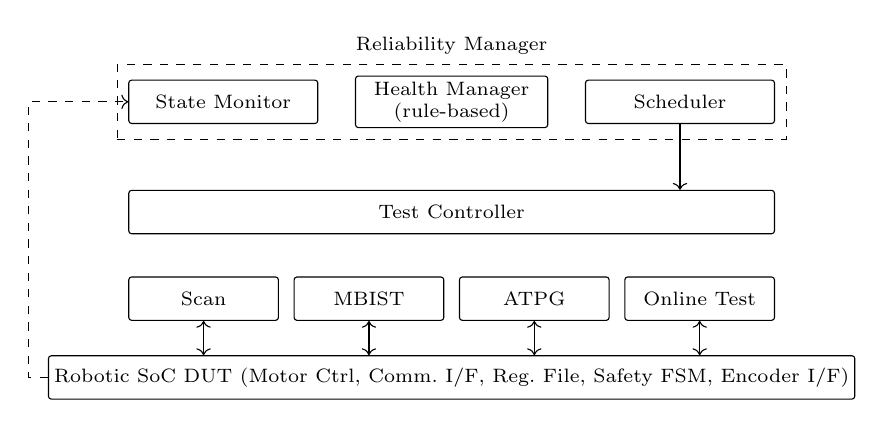
\begin{tikzpicture}[font=\scriptsize, box/.style={draw, rounded corners=1pt, align=center, inner sep=2pt, minimum height=0.55cm}]
\node[box, minimum width=8.2cm] (dut) at (0,0) {Robotic SoC DUT (Motor Ctrl, Comm.\ I/F, Reg.\ File, Safety FSM, Encoder I/F)};
\node[box, minimum width=1.9cm] (scan) at (-3.15,1.0) {Scan};
\node[box, minimum width=1.9cm] (mbist) at (-1.05,1.0) {MBIST};
\node[box, minimum width=1.9cm] (atpg) at (1.05,1.0) {ATPG};
\node[box, minimum width=1.9cm] (onl) at (3.15,1.0) {Online Test};
\node[box, minimum width=8.2cm] (tc) at (0,2.1) {Test Controller};
\node[box, minimum width=2.4cm] (sm) at (-2.9,3.5) {State Monitor};
\node[box, minimum width=2.4cm, text width=2.3cm] (hm) at (0,3.5) {Health Manager (rule-based)};
\node[box, minimum width=2.4cm] (sch) at (2.9,3.5) {Scheduler};
\node[draw, dashed, fit=(sm)(hm)(sch), inner sep=4pt, label={[font=\scriptsize]above:Reliability Manager}] (rm) {};
\foreach \x in {scan,mbist,atpg,onl} \draw[<->] (\x.south) -- (dut.north -| \x);
\draw[->] (sch.south) -- (sch.south |- tc.north);
\draw[->, dashed] (dut.west) -- ++(-0.25,0) |- (sm.west);
\end{tikzpicture}
\caption{Layered architecture positioning: existing DFT primitives (bottom) are invoked by a Test Controller whose decisions are, in the proposed direction, driven by a Reliability Manager fusing system state, rule-based health assessment, and criticality (dashed feedback path indicates aging/fault information flowing back from the DUT into the State/Health layer).}
\label{fig:arch}
\end{figure}

\begin{figure}[t]
\centering
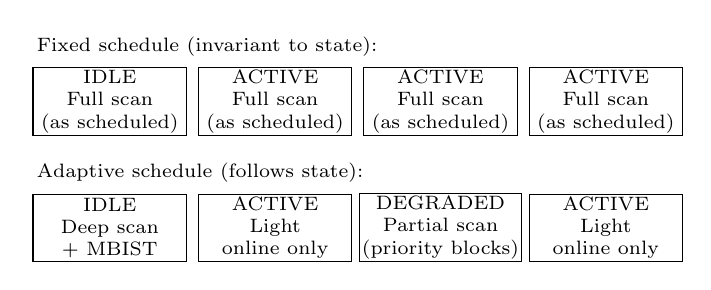
\begin{tikzpicture}[font=\scriptsize, c/.style={draw, align=center, minimum width=1.95cm, minimum height=0.85cm, inner sep=1pt}]
\node[anchor=west] at (0,1.5) {Fixed schedule (invariant to state):};
\foreach \i/\t in {0/IDLE,1/ACTIVE,2/ACTIVE,3/ACTIVE} \node[c] at (1.05+2.1*\i,0.8) {\t\\Full scan\\(as scheduled)};
\node[anchor=west] at (0,-0.1) {Adaptive schedule (follows state):};
\node[c] at (1.05,-0.8) {IDLE\\Deep scan\\+ MBIST};
\node[c] at (3.15,-0.8) {ACTIVE\\Light\\online only};
\node[c] at (5.25,-0.8) {DEGRADED\\Partial scan\\(priority blocks)};
\node[c] at (7.35,-0.8) {ACTIVE\\Light\\online only};
\end{tikzpicture}
\caption{Conceptual contrast between a fixed test schedule (top, invariant to operating state) and the proposed state-adaptive schedule (bottom, test depth/type follows the State Monitor and Health Manager outputs). No timing or coverage numbers are asserted; these are outputs of the project's own fault-injection evaluation, not of the surveyed literature.}
\label{fig:fixedadapt}
\end{figure}

\begin{figure}[t]
\centering
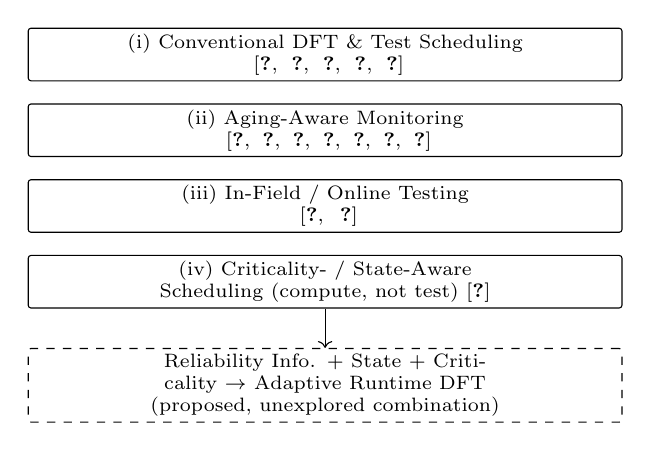
\begin{tikzpicture}[font=\scriptsize, b/.style={draw, rounded corners=1pt, align=center, text width=7.4cm, inner sep=2pt}, node distance=0.28cm]
\node[b] (a) {(i) Conventional DFT \& Test Scheduling\\ \cite{r1,r2,r3,r12,r11}};
\node[b, below=of a] (b) {(ii) Aging-Aware Monitoring\\ \cite{r4,r5,r13,r14,r6,r15,r7}};
\node[b, below=of b] (c) {(iii) In-Field / Online Testing\\ \cite{r9,r16}};
\node[b, below=of c] (d) {(iv) Criticality- / State-Aware Scheduling (compute, not test) \cite{r18}};
\node[b, dashed, below=0.5cm of d] (e) {Reliability Info. + State + Criticality $\rightarrow$ Adaptive Runtime DFT\\(proposed, unexplored combination)};
\draw[->] (d) -- (e);
\end{tikzpicture}
\caption{Literature taxonomy: the four layers surveyed (solid boxes, each independently mature and separately verified) and the unexplored combination this project targets (dashed box). No single verified source spans more than one solid layer with more than partial coverage of another (Table~\ref{tab:gap}).}
\label{fig:taxonomy}
\end{figure}

\section{Implementation of the Reliability-Aware DFT Architecture}
\label{sec:impl}
The proposed architecture was implemented as a mixed SystemVerilog and Python prototype to evaluate reliability-aware test scheduling for a robotic system-on-chip (SoC). The prototype consists of five functional blocks: a safety finite-state machine, motor controller, encoder interface, communication interface, and register file. The design integrates conventional design-for-test (DFT) mechanisms with a reliability manager that monitors operating conditions, maintains block-level health information, and selects tests according to the current operating state.

The DFT subsystem includes scan flip-flops and scan chains, a PODEM-based stuck-at ATPG flow, a March C$-$ memory-test controller, and a lightweight online test mechanism based on shadow comparison. The reliability manager comprises a state monitor, an aging model, a health manager, a priority engine, and a test scheduler. The implementation supports IDLE, ACTIVE, and DEGRADED operating states. In IDLE, the scheduler can perform full-scan testing and memory diagnostics; in ACTIVE, it favors lightweight online tests and scheduled testing; in DEGRADED, it increases diagnostic attention to flagged blocks and can escalate to a full-depth diagnostic when the available evidence is insufficient to justify recovery.

The adaptive scheduler implements the priority expression
\begin{equation*}
\begin{split}\mathrm{Priority}_i={}&w_1\mathrm{Crit}_i+w_2\mathrm{Health}_i+w_3\mathrm{Aging}_i\\&+w_4\mathrm{Faults}_i+w_5\mathrm{Mission}_i,\end{split}
\end{equation*}
where the terms represent block criticality, health, aging risk, fault history, and mission dependence, respectively. The five weights were set to unity in the reported experiments. Block criticality values, aging accumulation parameters, diagnostic thresholds, scheduling intervals, and mission-reliance profiles are configurable model parameters. Unless explicitly identified as part of the proposed policy, these values are implementation assumptions rather than parameters derived from physical silicon measurements.

\subsection{Diagnostic Evidence and Escalation}
The Phase~1 implementation adds three configurable mechanisms. First, the observability-aware evidence mechanism (\texttt{obs\_en}) records the depth required to resolve a detected failure. A passing diagnostic can clear unresolved evidence only when its test set provides sufficient coverage of the recorded failure class. An unknown failure class conservatively requires full-depth testing. This prevents a partial-scan pass from clearing a failure that requires a stronger diagnostic.

Second, the escalation mechanism (\texttt{esc\_en}) allows a flagged block requiring full-depth evidence to receive a full-scan diagnostic instead of another partial scan. The configured escalation interval is 10 scheduler ticks; this value is an experimental assumption and has not yet been optimized. Third, the stale-age mechanism (\texttt{stale\_en}) records when a block's age counter reaches its maximum representable value, preventing counter wraparound from incorrectly making an overdue block appear current. All three mechanisms are disabled by default, preserving the earlier reference configuration unless explicitly enabled.

\subsection{Experimental Setup}
The scheduler was evaluated using a Python reference model and SystemVerilog RTL. The experimental campaign uses a 600-tick synthetic mission trace, with 20,000 modeled cycles per tick, and a collapsed fault database containing 2,515 faults. The documented development seeds are 2024 for mission generation and 4242 for fault injection. Fault-detection decisions use precomputed test-detection tables for full scan, partial scan, MBIST, and online testing. The campaign evaluates one injected fault per episode and separately considers persistent faults and transient faults removed after 60 ticks.

Two types of experiment are distinguished. First-detection experiments evaluate which test first detects a fault under the scheduled test sequence. Closed-loop experiments additionally model diagnostic flag assertion, continued DEGRADED operation, escalation, and possible recovery after a transient fault is removed. These metrics are not interchangeable: detection of a fault does not by itself establish that the reliability manager can safely clear the resulting diagnostic evidence.

\subsection{Fairness Exemption and Service Bound}
The completed implementation adds an optional \texttt{fair\_unres\_en} parameter. When enabled, an overdue block that is not flagged is eligible for a priority-selected FULL+DIAG service even during mission-active DEGRADED operation while another block retains unresolved evidence. The exemption does not clear evidence, change escalation classification, or select a flagged block as healthy. The campaign configuration uses \texttt{overdue\_ticks}=150 and \texttt{fair\_gap}=4, so 154 ticks is a configured threshold-plus-gap criterion. Across the saved 2,515-episode campaign, the maximum observed post-flag healthy-block delay was 151 ticks (median 129, 95th percentile 148, zero observed delays above 154). This is an empirical result, not a formal guarantee: controller busy/overrun behavior, multiple unresolved faults, and arbitrary mission traces are not exhaustively proven.

\subsection{Reported Results}
In the saved single-seed closed-loop campaign, 2,451 of 2,515 persistent-fault episodes raised a diagnostic flag under the reference profile. The reference configuration cleared diagnostic flags while the injected fault remained present in 117 flagged episodes. Enabling observability-aware evidence reduced this count to zero. However, observability alone prevented recovery after transient faults were removed: none of the 2,440 flagged transient episodes recovered within the campaign. Adding escalation retained zero premature clearances and enabled recovery in 2,267 of those 2,440 episodes. The remaining 173 episodes ended without recovery within the modeled mission.

For persistent-fault episodes, mean modeled interruption cycles increased from 469,680 in the reference profile to 484,385 with observability plus the fairness exemption and 523,653 with observability, fairness, and escalation. These are increases of 3.1\% and 11.5\% relative to the reference. For transient episodes, the corresponding means are 72,344, 483,985, and 89,153 cycles. The fairness exemption is therefore evaluated as a service-availability safeguard, not as a guaranteed reduction in interruption cost.

\begin{table}[t]
\caption{Closed-loop results of the prototype (2,515 single-fault episodes; mission seed 2024, injection seed 4242; development seeds only)}
\label{tab:impl}
\centering\footnotesize
\setlength{\tabcolsep}{3pt}
\begin{tabular}{@{}lccc@{}}
\toprule
 & Reference & \texttt{obs\_en}+fair & \texttt{obs\_en}+fair+\texttt{esc\_en}\\
\midrule
\multicolumn{4}{@{}l}{\emph{Persistent faults}}\\
Flagged episodes & 2,451 & 2,451 & 2,451\\
Cleared while fault present & 117 & 0 & 0\\
Mean interruption cycles & 469,680 & 484,385 & 523,653\\
Change vs.\ reference & -- & +3.1\% & +11.5\%\\
\midrule
\multicolumn{4}{@{}l}{\emph{Transient faults (removed after 60 ticks)}}\\
Flagged episodes & 2,440 & 2,440 & 2,440\\
Cleared while fault present & 112 & 0 & 0\\
Mean interruption cycles & 72,344 & 483,985 & 89,153\\
Recovered after fault ended & 2,174 & 0 & 2,267\\
Flagged at end of mission & 155 & 2,440 & 173\\
\bottomrule
\end{tabular}
\end{table}

\begin{figure}[t]
\centering
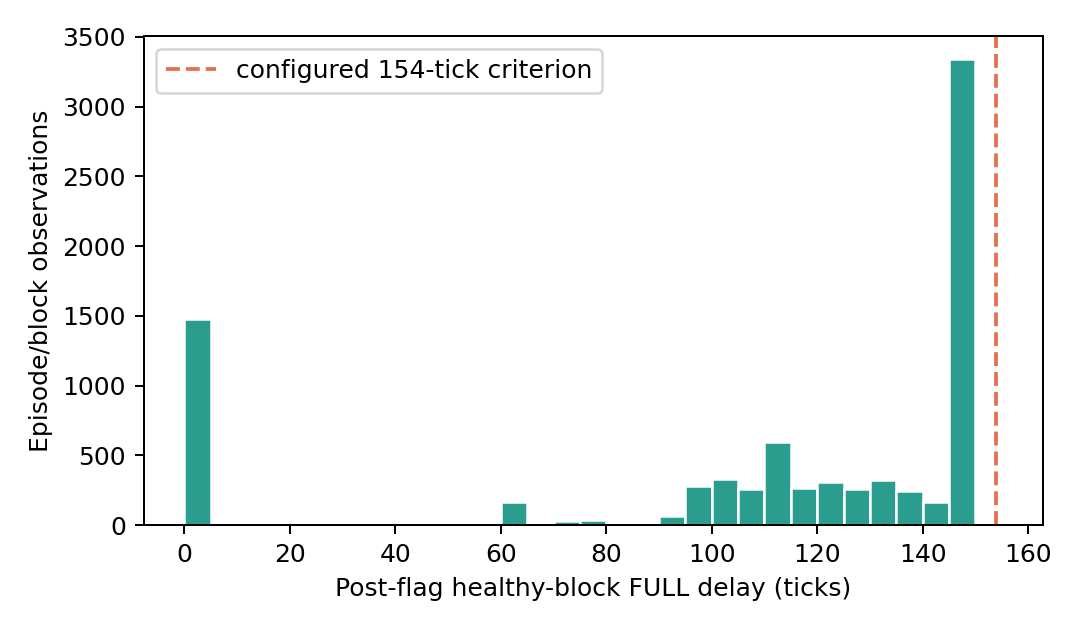
\includegraphics[width=\columnwidth]{fairness_delay_histogram.png}
\caption{Observed post-flag healthy-block FULL-service delays in the final seeded campaign. The dashed line is the configured 154-tick criterion; the maximum observed value is 151. This is an empirical distribution, not a formal proof.}
\label{fig:fairness-delay}
\end{figure}

\subsection{Scope and Limitations}
The results are from a behavioral model, one mission trace, one injection seed, and single-fault episodes. The RTL now propagates completed test failure classes into the Reliability Manager and exposes accepted/overrun controller handshakes; the fairness parameter is configurable at the SoC top level, but the saved campaign remains a Python closed-loop experiment with scripted RTL equivalence rather than a full multi-seed integrated-SoC campaign. The aging model is an activity-accumulation abstraction; it does not simulate calibrated NBTI, HCI, or other measured physical aging processes. Diagnostic test-class information is supplied by the campaign or testbench rather than generated by an integrated physical test controller. The reported results establish functional behavior within the modeled fault and detection tables; they do not establish silicon-level reliability, power, timing, area, or universal superiority over fixed-period testing. A multi-seed evaluation, fixed-period and adaptive-policy comparisons under matched conditions, formal or exhaustive fairness proof, and technology-aware hardware-cost measurements remain necessary for broader performance claims. The STA-based critical-path ranking and aging-sensor placement of Layer~B (Section~IX) are not implemented in the prototype.

\section{Open Challenges and Future Research Directions}
Grounded in the gaps identified in Sections VIII--IX, the following directions are forward-looking research proposals rather than established literature findings, and are labeled as such:
\begin{itemize}
\item \textbf{Calibrating a fused priority score.} Eq.~(2)'s weights $w_1,\ldots,w_5$ are, at present, undetermined; a systematic sensitivity study against the fault-injection campaign in the project's evaluation plan is needed before any claim of scheduler quality can be made.
\item \textbf{Extending aging-sensor placement methods to a robotic duty-cycle model.} The G\'omez--Champac, V\'azquez et al., and Koneru et al. methodologies were developed and evaluated on general digital logic \cite{r4,r13,r6}, not against an IDLE/ACTIVE/DEGRADED duty-cycle model; whether their stress-probability assumptions transfer to a robotic controller's duty cycle is an open, testable question rather than an assumed result.
\item \textbf{Reconciling periodic and continuous online-test paradigms.} The patented lifecycle-triggered controller \cite{r9} and the fully concurrent CBIST approach \cite{r16} represent two different points on a periodicity-vs.-intrusiveness spectrum; combining a criticality-aware trigger (Section~IX) with a concurrency mechanism for the ACTIVE state specifically is an integration question this survey has not seen addressed for synchronous robotic-controller logic.
\item \textbf{Machine-learning-assisted reliability prediction and reinforcement-learning-based scheduling} are plausible extensions of the rule-based Health Manager and Scheduler described here, but are explicitly out of scope for the frozen project architecture (Section~IX) and are not supported, in this survey, by any verified source that applies them to this specific combination of aging, state, and criticality; they are listed here only as directions, not as claims.
\item \textbf{Radiation/soft-error-aware extensions.} Trikarenos's structural (TCLS/ECC) approach to soft-error tolerance \cite{r8} is complementary to, not a substitute for, the scheduled-diagnostic approach surveyed here; combining structural redundancy with reliability-aware scheduling for the residual, uncorrected fault population is an open direction.
\end{itemize}

\section{Research Gap and Positioning of the Proposed Architecture}
\label{sec:gap}
Table~\ref{tab:gap} constructs a literature-gap matrix across the major sources verified for this survey, using the ten dimensions specified for this analysis, and Figure~\ref{fig:chain} restates the same argument as a research-evolution chain. A checkmark (\ck) indicates the dimension is directly addressed and evaluated by the source; ``partial'' indicates the dimension is present but limited in scope (e.g., addressed only for one axis, or asserted but not empirically evaluated in the verified source); an em-dash indicates the dimension is not addressed.

\begin{table*}[t]
\caption{Literature Gap Matrix}
\label{tab:gap}
\centering\scriptsize
\setlength{\tabcolsep}{3pt}
\begin{tabularx}{\textwidth}{@{}lcccccccccX@{}}
\toprule
Source & Manuf.\ DFT & In-field & Aging & Sys.\ State & Criticality & Adaptive Sched. & Fault Hist. & Online & Robotic/ Autonomous & Research Gap Noted\\
\midrule
\cite{r1} & \ck & -- & -- & -- & -- & -- & -- & -- & -- & Manufacturing-only\\
\cite{r2} & \ck & -- & -- & -- & -- & -- & -- & -- & -- & Static schedule only\\
\cite{r3} & \ck & -- & -- & Partial (thermal) & -- & -- & -- & -- & -- & State limited to temperature\\
\cite{r11} & \ck & -- & -- & -- & -- & -- & -- & -- & -- & Power substrate, not scheduling\\
\cite{r4,r5,r13,r14} & Partial & -- & \ck & -- & -- & -- & -- & -- & -- & Sensing/placement, no scheduling\\
\cite{r6,r15} & Partial & \ck (sensing) & \ck & -- & -- & -- & -- & \ck & -- & Signal only, no decision layer\\
\cite{r7} & \ck & -- & \ck & -- & -- & -- & -- & -- & -- & Production screening only\\
\cite{r9} & -- & \ck & -- & -- & -- & Partial (periodic) & -- & Partial & Automotive & Periodic, not state-fused\\
\cite{r16} & -- & \ck & -- & -- & -- & -- & -- & \ck & -- & Async logic only\\
\cite{r8} & -- & \ck (redundancy) & -- & -- & -- & -- & Implicit & \ck & Space/ automotive & Structural, not scheduled\\
\cite{r18} & -- & -- & -- & \ck & \ck & \ck & -- & \ck & Automotive (always-active) & Compute, not test; no idle model\\
\bottomrule
\end{tabularx}
\end{table*}

\begin{figure}[t]
\centering
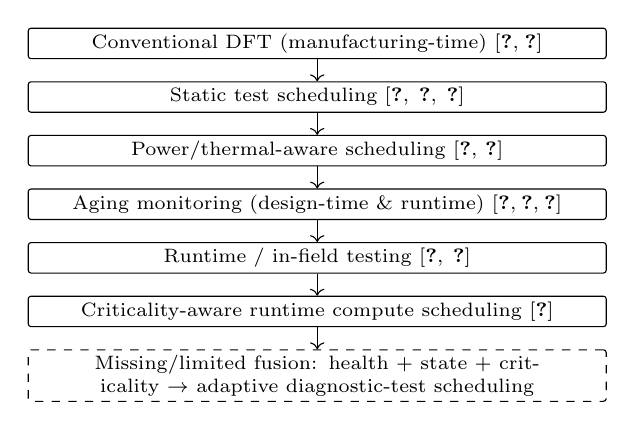
\begin{tikzpicture}[font=\scriptsize, b/.style={draw, rounded corners=1pt, align=center, text width=7.2cm, inner sep=2pt}, node distance=0.28cm]
\node[b] (a) {Conventional DFT (manufacturing-time) \cite{r1,r2}};
\node[b, below=of a] (b) {Static test scheduling \cite{r2,r3,r12}};
\node[b, below=of b] (c) {Power/thermal-aware scheduling \cite{r11,r3}};
\node[b, below=of c] (d) {Aging monitoring (design-time \& runtime) \cite{r4,r13,r6}};
\node[b, below=of d] (e) {Runtime / in-field testing \cite{r9,r16}};
\node[b, below=of e] (f) {Criticality-aware runtime compute scheduling \cite{r18}};
\node[b, dashed, below=of f] (g) {Missing/limited fusion: health + state + criticality $\rightarrow$ adaptive diagnostic-test scheduling};
\foreach \x/\y in {a/b,b/c,c/d,d/e,e/f,f/g} \draw[->] (\x) -- (\y);
\end{tikzpicture}
\caption{Research-evolution chain underlying the gap statement of Section~\ref{sec:gap}: each stage is independently established in the verified literature; the final, dashed stage is not demonstrated by any single verified source and is the project's proposed research direction, not a literature finding.}
\label{fig:chain}
\end{figure}

\textbf{Reading the matrix.} No single verified source populates more than three of the ``Aging,'' ``System State,'' ``Criticality,'' and ``Adaptive Scheduling'' columns simultaneously, and no source combines any of these with a test/diagnostic scheduling objective and a genuine idle/active/degraded duty-cycle model. Based on the surveyed literature, the following positioning statements can be made with the appropriate caution:
\begin{enumerate}
\item Manufacturing-time DFT architecture and scheduling (Section~II) is mature, static, and not itself in dispute; it is correctly treated in the project's evaluation plan as the non-novel baseline against which any adaptive scheme must be measured.
\item Aging-aware sensing (Section~IV) is mature as a measurement technology but, in the sources verified here, is not coupled to a scheduling decision.
\item In-field self-test triggering exists in patented industrial practice \cite{r9}, which means periodic/lifecycle-triggered in-field self-test is prior art and cannot itself be claimed as the contribution; what remains open is whether the trigger can be made continuously state-and-health-fused rather than periodic.
\item Criticality-and-state-aware runtime scheduling is demonstrated, and rigorously evaluated, for compute tasks on automotive SoCs \cite{r18}; to the best of the authors' knowledge based on the sources examined for this survey, an analogous scheduler for test/diagnostic tasks, fused with an aging/health signal, and evaluated against a robotic (rather than always-substantially-active automotive) duty-cycle model including a genuine idle state, is not demonstrated in the literature surveyed here.
\item The specific combination stated as this project's novelty statement -- Reliability Information + System State + Criticality $\rightarrow$ Adaptive Runtime DFT -- is therefore best characterized as a genuinely unexplored combination of independently mature components (Sections II--VII), rather than as a new component in itself. This is a narrower and more defensible claim than asserting that any individual piece (aging monitoring, in-field self-test, or criticality-aware scheduling) is novel, since each of those pieces individually is not.
\end{enumerate}

\section{Conclusion}
This paper examined conventional SoC DFT and test scheduling, low-power DFT, aging-aware reliability monitoring, in-field/online testing, and criticality-and-state-aware scheduling of non-test workloads, drawing exclusively on sources whose existence, authorship, venue, and (where applicable) reported results were verified against IEEE Xplore, arXiv, ACM/Springer bibliographic records, and the U.S. Patent database. Each family of techniques was shown to address one or two axes of the reliability-testing problem for autonomous robotic SoCs -- manufacturing efficiency, aging measurement, in-field triggering, or criticality-aware runtime decision-making -- without any single verified source jointly addressing aging, operating state, criticality, and test (as opposed to compute) scheduling for a genuinely idle-capable robotic duty cycle. On this basis, a reliability-aware, state-adaptive DFT scheduler that fuses these signals is positioned as an unexplored combination of existing, individually mature components. A behavioral prototype of the scheduler (Section~\ref{sec:impl}) exercises this combination in a single-seed, single-mission, single-fault setting. The completed package adds a bounded fairness regression, explicit result-class plumbing, generic synthesis counts, and reproducibility metadata, but does not establish silicon-level reliability, physical PPA, or a universal service deadline.

\section*{Acknowledgment}
The numerical results reported for this prototype are generated from the machine-readable artefacts in \\texttt{results_final/}; prior-work claims are attributed to the cited sources.

\begin{thebibliography}{99}
\bibitem{r1} S. K. Goel and E. J. Marinissen, ``Effective and efficient test architecture design for SOCs,'' in \emph{Proc. IEEE Int. Test Conf. (ITC)}, Baltimore, MD, USA, 2002, pp. 529--538.
\bibitem{r2} K. Chakrabarty, ``Test scheduling for core-based systems using mixed-integer linear programming,'' \emph{IEEE Trans. Comput.-Aided Design Integr. Circuits Syst.}, vol. 19, no. 10, pp. 1163--1174, 2000.
\bibitem{r3} Z. He, Z. Peng, P. Eles, P. Rosinger, and B. M. Al-Hashimi, ``Thermal-aware SoC test scheduling with test set partitioning and interleaving,'' in \emph{Proc. 21st IEEE Int. Symp. Defect and Fault-Tolerance in VLSI Systems (DFT)}, Washington, DC, USA, 2006, pp. 477--485.
\bibitem{r4} A. F. G\'omez, L. B. Poehls, F. Vargas, and V. H. Champac, ``An early prediction methodology for aging sensor insertion to assure safe circuit operation due to NBTI aging,'' in \emph{Proc. IEEE VLSI Test Symp. (VTS)}, 2015, pp. 1--6.
\bibitem{r5} A. F. G\'omez and V. H. Champac, ``Early selection of critical paths for reliable NBTI aging-delay monitoring,'' \emph{IEEE Trans. Very Large Scale Integr. (VLSI) Syst.}, vol. 24, no. 7, pp. 2438--2448, 2016.
\bibitem{r6} A. Koneru, A. Vijayan, K. Chakrabarty, and M. B. Tahoori, ``Fine-grained aging prediction based on the monitoring of run-time stress using DFT infrastructure,'' in \emph{Proc. IEEE/ACM Int. Conf. Computer-Aided Design (ICCAD)}, 2015, pp. 51--58.
\bibitem{r7} L. Yu, J. Ren, X. Lu, and X. Wang, ``NBTI and HCI aging prediction and reliability screening during production test,'' \emph{IEEE Trans. Comput.-Aided Design Integr. Circuits Syst.}, vol. 39, no. 10, pp. 3000--3011, 2020.
\bibitem{r8} M. Rogenmoser, P. Wiese, B. E. Forlin, F. K. G\"urkaynak, P. Rech, A. Menicucci, M. Ottavi, and L. Benini, ``Trikarenos: Design and experimental characterization of a fault-tolerant 28nm RISC-V-based SoC,'' arXiv:2407.05938 [physics.ins-det], 2024.
\bibitem{r9} A. Jain, N. B. Singh, R. Gulati, P. Bhuyan, R. K. Kinger, and R. Averbuj, ``In-field self-test controller for safety critical automotive use cases,'' US Patent 10,481,202 B2, 2019.
\bibitem{r10} International Organization for Standardization, ``ISO 26262: Road vehicles -- functional safety,'' ISO Standard 26262, 2018.
\bibitem{r11} S. Seo, Y. Lee, H. Lim, J. Lee, H. Yoo, Y. Kim, and S. Kang, ``Scan chain reordering-aware x-filling and stitching for scan shift power reduction,'' in \emph{Proc. 24th IEEE Asian Test Symp. (ATS)}, 2015, pp. 1--6.
\bibitem{r12} P. Rosinger, B. M. Al-Hashimi, and K. Chakrabarty, ``Thermal-safe test scheduling for core-based system-on-chip integrated circuits,'' \emph{IEEE Trans. Comput.-Aided Design Integr. Circuits Syst.}, vol. 25, no. 11, pp. 2502--2512, 2006.
\bibitem{r13} J. C. V\'azquez, V. H. Champac, J. Semi\~ao, I. C. Teixeira, M. B. Santos, and J. P. Teixeira, ``Process variations-aware statistical analysis framework for aging sensors insertion,'' \emph{J. Electronic Testing: Theory and Applications}, vol. 29, no. 3, pp. 289--299, 2013.
\bibitem{r14} F. Firouzi, F. Ye, K. Chakrabarty, and M. B. Tahoori, ``Aging- and variation-aware delay monitoring using representative critical path selection,'' \emph{ACM Trans. Design Autom. Electron. Syst.}, vol. 20, no. 3, pp. 39:1--39:23, 2015.
\bibitem{r15} A. Vijayan, A. Koneru, S. Kiamehr, K. Chakrabarty, and M. B. Tahoori, ``Fine-grained aging-induced delay prediction based on the monitoring of run-time stress,'' \emph{IEEE Trans. Comput.-Aided Design Integr. Circuits Syst.}, vol. 37, no. 5, pp. 1064--1075, 2018.
\bibitem{r16} J. Maier and A. Steininger, ``Online test vector insertion: A concurrent built-in self-testing (CBIST) approach for asynchronous logic,'' in \emph{Proc. 17th IEEE Int. Symp. Design and Diagnostics of Electronic Circuits \& Systems (DDECS)}, 2014, pp. 33--38.
\bibitem{r17} M. Rogenmoser, P. Wiese, B. E. Forlin, F. K. G\"urkaynak, P. Rech, A. Menicucci, M. Ottavi, and L. Benini, ``Trikarenos: Design and experimental characterization of a fault-tolerant 28-nm RISC-V-based SoC,'' \emph{IEEE Trans. Nucl. Sci.}, vol. 72, no. 8, pp. 2783--2792, 2025.
\bibitem{r18} A. Amarnath, S. Pal, H. Kassa, A. Vega, A. Buyuktosunoglu, H. Franke, J.-D. Wellman, R. Dreslinski, and P. Bose, ``HetSched: Quality-of-mission aware scheduling for autonomous vehicle SoCs,'' arXiv:2203.13396 [cs.AR], 2022.
\bibitem{r19} IEEE, ``IEEE standard testability method for embedded core-based integrated circuits,'' IEEE Std 1500-2005, 2005.
\end{thebibliography}
\end{document}
